% !TEX encoding = UTF-8
% !TEX TS-program = pdflatex
% !TEX root = ../tesi.tex
% !TEX spellcheck = it-IT

%*************************************************************
\chapter{La localizzazione con RSSI}
\label{cap:localizzazione-con-rssi}
%*************************************************************

Una delle tecniche di localizzazione più comuni per la stima della posizione in ambiente indoor è la tecnica \emph{Anchor based}. Nella tecnica Anchor based un sottoinsieme di nodi della rete, chiamati \emph{anchor} o \emph{beacon}, sono a conoscenza della loro posizione, ottenuta grazie al GPS o avendo stabilito un sistema di coordinate predefinite. Gli altri nodi (\emph{target}) usano le informazioni di posizione dai nodi anchor per determinare la propria posizione. Il ranging tra i beacon e gli altri nodi può essere ottenuto con
\begin{itemize}
	
	\item
	interazione diretta (Single-Hop)
	
	\item 
	indirettamente, per mezzo di nodi intermedi (Multi-Hop)
	
\end{itemize}
Per quanto riguarda il processo di localizzazione, questo può essere affrontato usando la tecnica \emph{Range based}. Nella tecnica Range based vengono effettuate una serie di misurazioni per conoscere la distanza tra beacon e target (\emph{ranging}). A questo punto, con l’algoritmo di trilaterazione (vedi paragrafo \ref{par:trilaterazione}) è possibile stimare la posizione dei nodi target.

\section{Ranging: stima della distanza}
\label{par:ranging}
Per stimare la distanza tra beacon e target si è utilizzata una tecnica di tipo range-based dato che è una tra le tecniche più economiche, essendo l'economicità uno dei requisiti fondamentali e maggiormente apprezzabili quando si va a verificare un'applicazione.
Il primo passo da affrontare in un processo di localizzazione di questo tipo è il ranging.
Il ranging tra due nodi è dunque la tecnica utilizzata da questi per determinare la distanza che si separa. Una delle tecniche su cui ci si può basare per la stima della distanza è la valutazione dell'intensità del segnale ricevuto (RSSI).

\section{Received Signal Strenght (RSSI)}
Valutando l'intensità di un segnale ricevuto è possibile stimare la distanza dalla stazione che l'ha trasmesso. Nel caso di dispositivi Bluetooth quello che si va ad utilizzare è un indicatore di potenza, l'RSSI (Received Signal Strenght Indicator), il quale indica una stima della potenza del segnale ricevuto misurato in dBm. Per andare a valutare la distanza dalla quale questo segnale è stato trasmesso si può utilizzare l'equazione di Friis:

\begin{equation}
\label{eq:friis}
P_R=P_T\frac{G_T G_R \lambda^2}{(4\pi)^2 d^n}
\end{equation}

dove:
\begin{itemize}
	
	\item $P_R$ è la potenza del segnale ricevuto in Watt
	
	\item $P_T$ è la potenza del segnale trasmesso in Watt
	
	\item $G_R$ è il guadagno dell'antenna ricevente
	
	\item $G_T$ è il guadagno dell'antenna trasmittente
	
	\item $\lambda$ è la lunghezza d'onda dove $\lambda=c/f$ dove $c$ è la velocità della luce \\ ($299792458\;m/s$) e $f$ è la frequenza
	
	\item $d$ è la distanza in metri
	
	\item $n$ è la costante di propagazione del segnale, detto anche esponente di propagazione, dipende dall'ambiente in cui ci si trova
	
\end{itemize}

Risulta molto utile, dal punto di vista pratico la seguente formula, che ci permette di convertire la potenza da Watt a dBm, dal momento che l’indicatore RSSI è solitamente espresso in dBm.
\begin{equation}
\label{eq:p-dbm}
P[dBm]=10 \cdot log_{10}(P[W] \cdot 10^3)
\end{equation}

Per motivi di semplicità, è possibile combinare assieme la \ref{eq:friis} e la \ref{eq:p-dbm}. Applicando le proprietà dei logaritmi, si ottiene la seguente formula:
\begin{equation}
RSSI=-(10 \cdot n \cdot log_{10}d - A)
\end{equation}

Dove $A$ è la potenza del segnale ricevuto, in dBm, alla distanza di riferimento di un metro e $n$ è la costante di propagazione del segnale.

In figura \ref{fig:andamento-potenza-distanza} è rappresentato l'andamento ideale dell'indicatore RSSI in ambiente aperto ($n=2$, $A=-40dBm$).

A questo punto è conveniente aggiustare la relazione sopra scritta:
\begin{equation}
log_{10}d = \frac{A - RSSI}{10 \cdot n}
\end{equation}

Infine, isolando la distanza:
\begin{equation}
d = 10^{(\frac{A - RSSI}{10 \cdot n})}
\end{equation}

Quest'ultima formula, ci permette quindi di calcolare la distanza tra due nodi conoscendo il valore di RSSI ed i parametri $A$ e $n$.

\begin{figure}[htp]
	\centering
	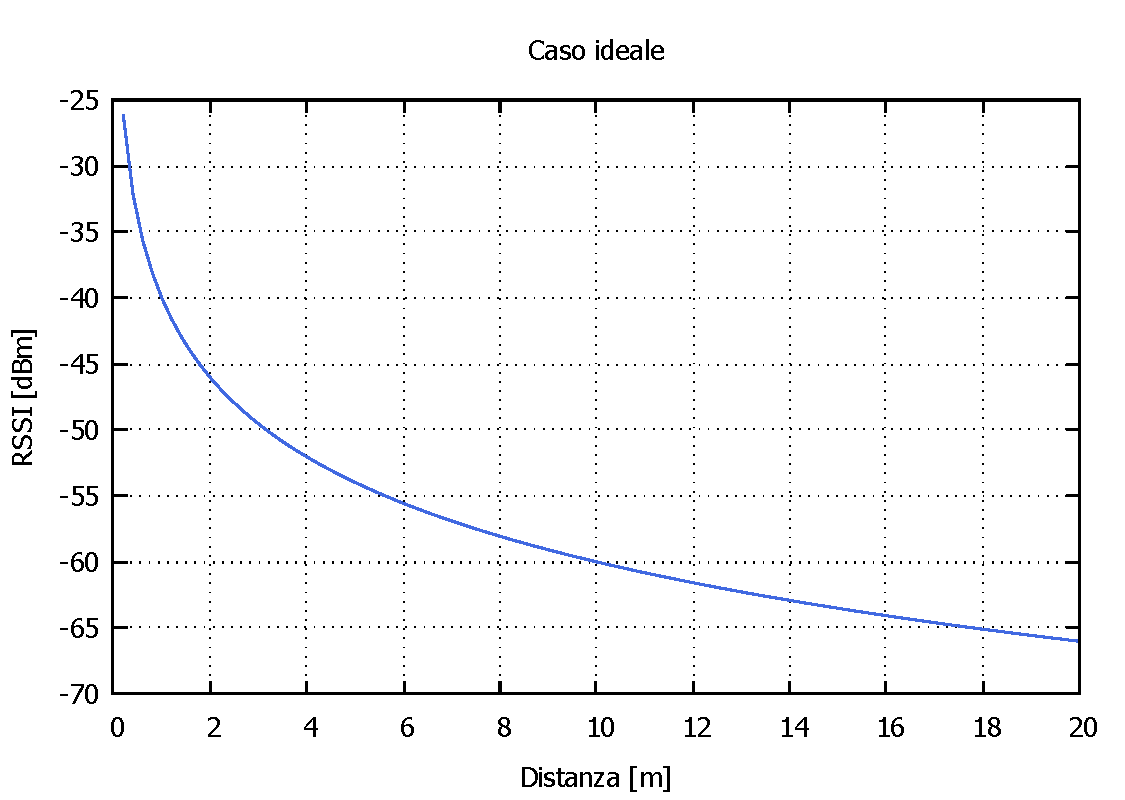
\includegraphics[height=\textheight/3]{andamento-potenza-distanza}
	\caption{Andamento ideale della potenza ricevuta in funzione della distanza}
	\label{fig:andamento-potenza-distanza}
\end{figure}

\section{L'algoritmo di trilaterazione}
\label{par:trilaterazione}
Uno degli algoritmi più utilizzati per la localizzazione è l'algoritmo di trilaterazione. Questo algoritmo non necessita di mappature del segnale radio, riducendo così fortemente il tempo richiesto per la calibrazione e, allo stesso tempo, garantendo maggior flessibilità al dinamismo e alle modifiche dell'ambiente.
La trilaterazione è un algoritmo di localizzazione basato su principi geometrici. Per poter calcolare la posizione di un dispositivo si deve conoscere la distanza dal dispositivo da ogni beacon. Vengono quindi disegnati dei cerchi avente come centro le coordinate del nodo riferimento e raggio uguale alla distanza stimata. Idealmente, il nodo target si trova nel punto di intersezione tra i tre cerchi come mostrato in figura \ref{fig:trilaterazione-caso-ideale}. Sapendo che ogni circonferenza è descritta dall'equazione
\[
(x - x_i)^2 - (y - y_i)^2 = r_i^2
\]
con $(x_i , y_i)$ coordinate dei vari centri e $r_i$ raggio del cerchio i-esimo, per trovare l'intersezione basta risolvere il seguente sistema:
\begin{equation}
\begin{cases}
\label{eq:sistema-trilaterazione}
(x-x_1)^2 + (y-y_1)^2 = r_1^2 \\
(x-x_2)^2 + (y-y_2)^2 = r_2^2 \\
(x-x_3)^2 + (y-y_3)^2 = r_3^2
\end{cases}
\end{equation}

\begin{figure}[htp]
	\centering
	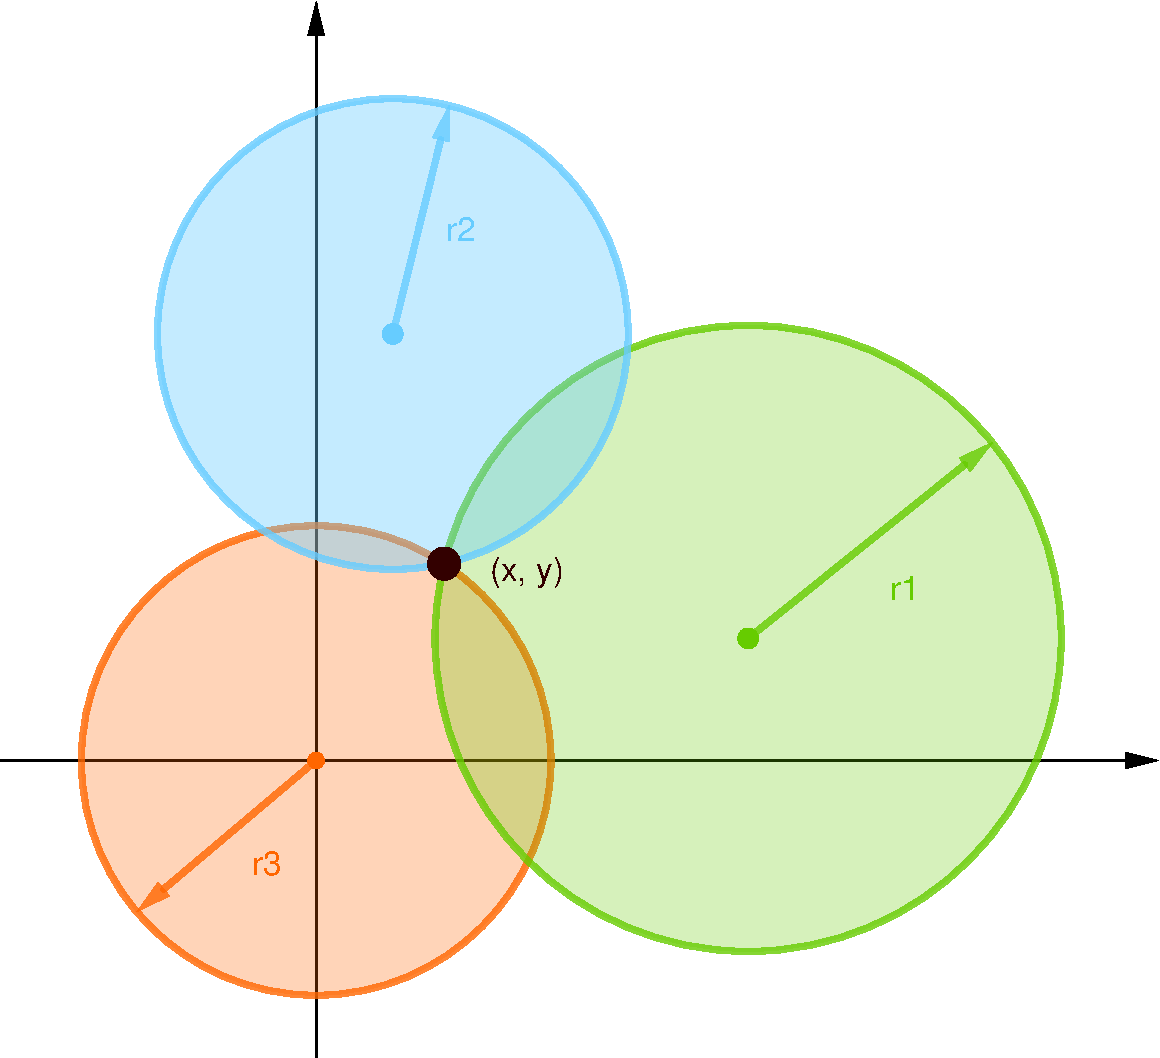
\includegraphics[height=\textheight/3]{trilaterazione-caso-ideale}
	\caption{Le coordinate del nodo target si trovano nel punto di intersezione dei tre cerchi}
	\label{fig:trilaterazione-caso-ideale}
\end{figure}

In pratica, tuttavia, le stime della distanza non sono mai così perfette e non viene quasi mai ottenuto un unico punto come intersezione. È più probabile che il nodo target si trovi all'interno di un’area di intersezione tra i cerchi, o è addirittura possibile che i cerchi non si tocchino. Per ovviare a questi inconvenienti si utilizzano dei piccoli accorgimenti al metodo tradizionale della Trilaterazione. Questo metodo che andremo a descrivere viene realizzato iterativamente per tutti e tre i nodi beacon.
\begin{enumerate}
	
	\item Vengono disegnati due cerchi attorno a due nodi beacon a scelta;
	
	\item Se il punto di intersezione è unico, si salvano le coordinate di questo;
	
	\item Se i due cerchi non si toccano, vengono aumentati i raggi in maniera proporzionale in modo che si tocchino in un unico punto;
	
	\item Se i due cerchi si toccano in due punti, viene considerato quello che ha distanza dal terzo nodo beacon più vicina alla stima della distanza calcolata per questo nodo;
	
	\item Alla fine di questo procedimento, iterato per tutti e tre i nodi, viene calcolata la media delle coordinate, che corrispondono alla posizione stimata del nodo.
	
\end{enumerate}
Questo algoritmo è leggermente più complesso, almeno in linea di principio, ma offre performance migliori. In figura \ref{fig:trilaterazione-raffinamento-passo-1}, figura \ref{fig:trilaterazione-raffinamento-passo-2} e figura \ref{fig:trilaterazione-raffinamento-passo-3} è mostrato come opera questo adattamento dell’algoritmo di Trilaterazione.

\begin{figure}[htp]
	\centering
	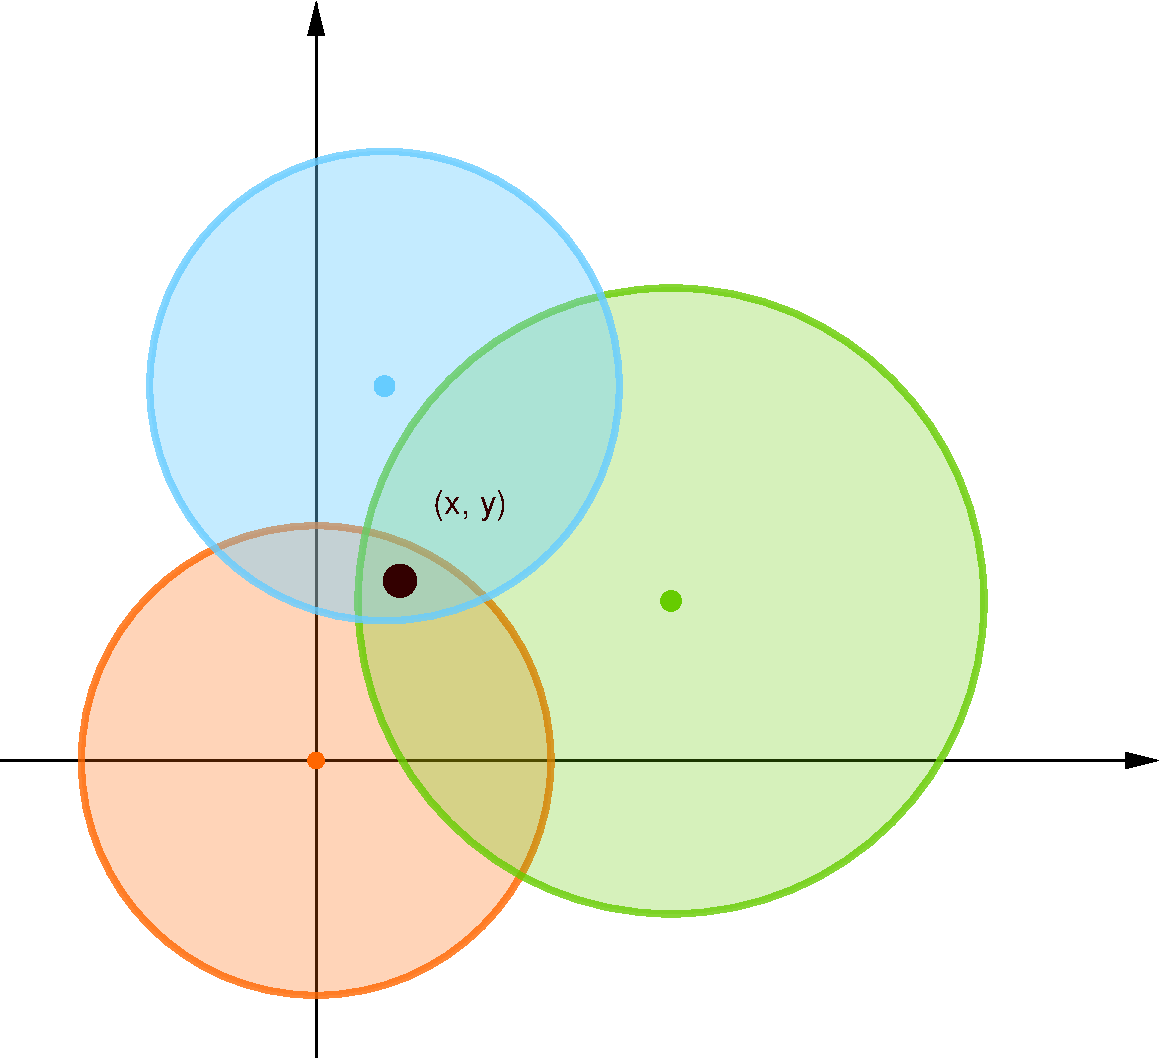
\includegraphics[height=\textheight/3]{trilaterazione-raffinamento-passo-1}
	\caption{Esempio del caso in cui il punto di intersezione non sia unico.}
	\label{fig:trilaterazione-raffinamento-passo-1}
\end{figure}

\begin{figure}[htp]
	\centering
	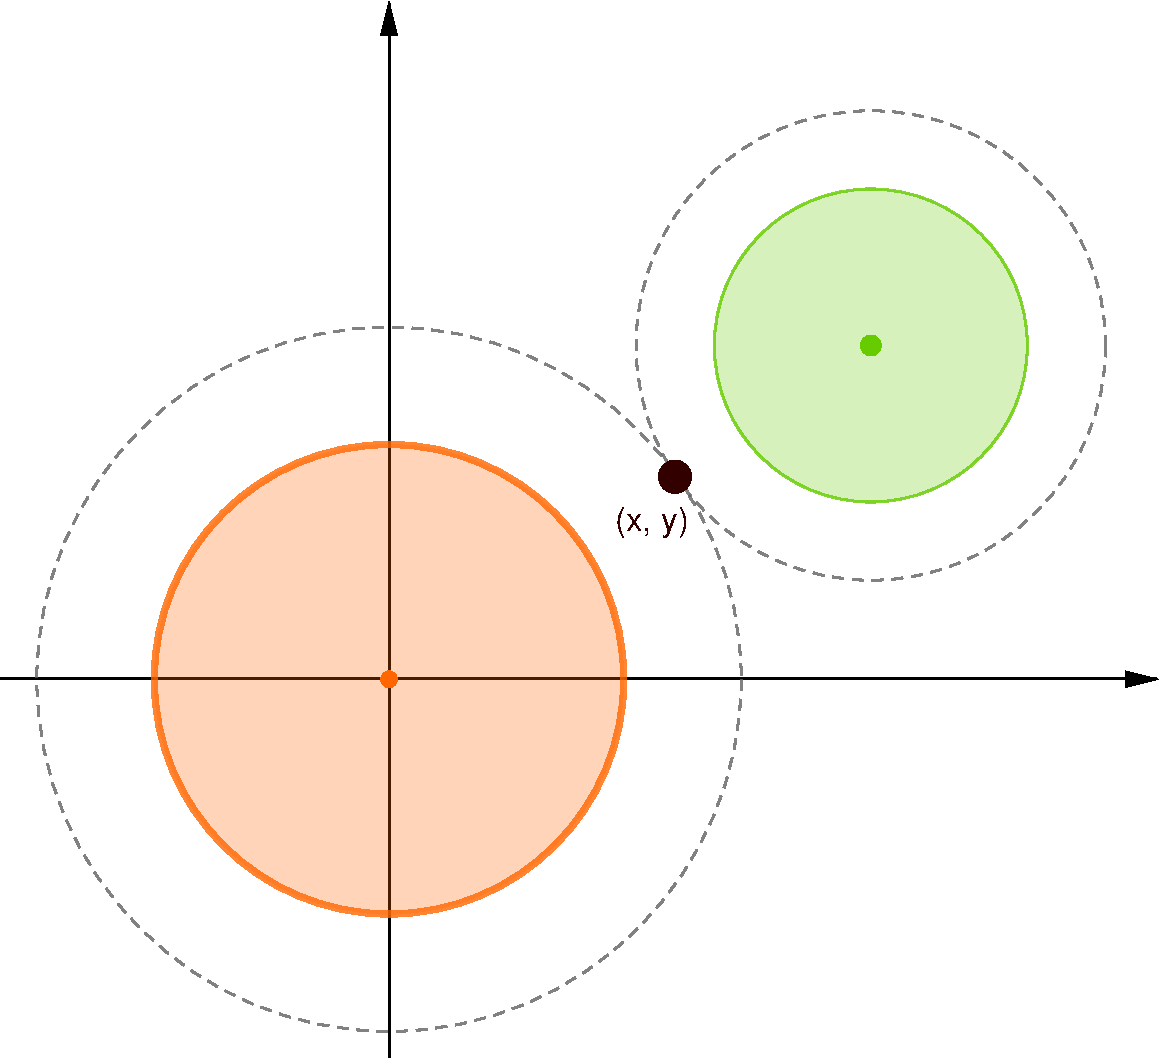
\includegraphics[height=\textheight/3]{trilaterazione-raffinamento-passo-2}
	\caption{Esempio del caso in cui i cerchi non si tocchino. Vengono aumentati i raggi in maniera proporzionale fin quando non si raggiunge il punto di incontro.}
	\label{fig:trilaterazione-raffinamento-passo-2}
\end{figure}

\begin{figure}[htp]
	\centering
	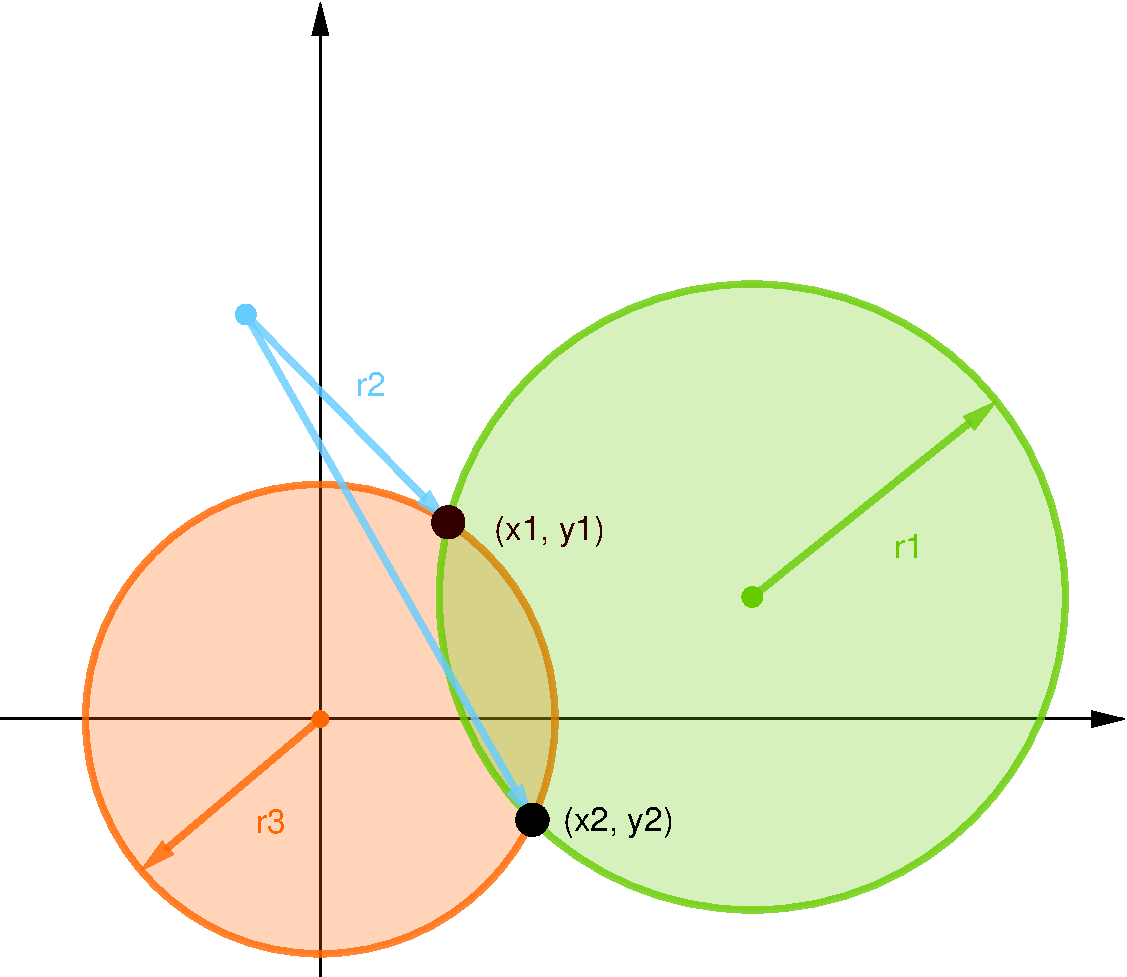
\includegraphics[height=\textheight/3]{trilaterazione-raffinamento-passo-3}
	\caption{Esempio del caso in cui vi siano due punti di intersezione. Il punto tenuto in considerazione è quello con distanza più vicina a quella stimata.}
	\label{fig:trilaterazione-raffinamento-passo-3}
\end{figure}